\documentclass[3p,12pt,times,authoryear]{elsarticle}
\usepackage{lineno,hyperref}
\usepackage{tikz}

%\biboptions{longnamesfirst,angle,semicolon}


%\bibliographystyle{unsrt}
%\bibliographystyle{plain}
%
%\bibliographystyle{elsarticle-num}
%
%\bibliographystyle{elsarticle-harv}
%
%\bibliographystyle{elsarticle-num-names}

%\bibliographystyle{model4-names}
\bibliographystyle{model5-names}

%行间距
\renewcommand{\baselinestretch}{1.1}\normalsize
%\setlength{\parskip}{1em} % 段间距


\begin{document}
	\begin{frontmatter}
		\title{This is a specimen title \tnoteref{t1,t2}}
		\tnotetext[t1]{This document is the results of the research
			project funded by the National Science Foundation.}
		\tnotetext[t2]{The second title footnote which is a longer
			text matter to fill through the whole text width and
			overflow into another line in the footnotes area of the
			first page.}
		\author[1]{Jos Migchielsen \corref{cor1}%
			\fnref{fn1}}
		\ead{J.Migchielsen@elsevier.com}
		\author[2]{CV Radhakrishnan \fnref{fn2,fn3}}
		\ead{cvr@sayahna.org}
		\author[3]{CV Rajagopal \fnref{fn1,fn3}}
		\ead[url]{www.stmdocs.in}
		\cortext[cor1]{Corresponding author}
		\fntext[fn1]{This is the first author footnote.}
		\fntext[fn2]{Another author footnote, this is a very long
			footnote and it should be a really long footnote. But this
			footnote is not yet sufficiently long enough to make two
			lines of footnote text.}
		\fntext[fn3]{Yet another author footnote.}
		\address[1]{Elsevier B.V., Radarweg 29, 1043 NX Amsterdam,
			The Netherlands}
		\address[2]{Sayahna Foundations, JWRA 34, Jagathy,
			Trivandrum 695014, India}
		\address[3]{STM Document Engineering Pvt Ltd., Mepukada,
			Malayinkil, Trivandrum 695571, India}
		\begin{abstract}
			In this paper, we propose ex-ante characteristics that predict the drop in risk-adjusted performance
			out-of-sample for a large set of stock anomalies published in finance and accounting
			academic journals. Our set of predictors is generated by hypotheses of OOS decay put forward
			by McLean and Pontiff (2016): arbitrage capital flowing into newly published strategies and
			in-sample overfitting linked to multiple hypothesis testing. The year of publication alone
			compatible with both hypotheses—explains 30\% of the variance of Sharpe decay across factors:
			Every year, the Sharpe decay of newly-published factors increases by 5ppt. The other
			important variables are directly related to overfitting: the number of operations required to
			calculate the signal and two measures of sensitivity of in-sample Sharpe to outliers together
			add another 15\% of explanatory power. Some arbitrage-related variables are statistically significant,
			but their predictive power is marginal
		\end{abstract}
		\begin{keyword}
			\texttt{elsarticle.cls}\sep \LaTeX\sep Elsevier \sep template
		\end{keyword}
	\end{frontmatter}
%	\linenumbers
	\section{Introduction}
	Although quadrupole excitons (QE) in cuprous oxide crystals are good candidates for BEC due to their narrow\cite{ISI:000614045200001}
	line-width and long life-time there are some factors impeding BEC Assume some density of quadrupole 1S excitons
	created by an external laser pulse\cite{ISI:000614045200001}. The corresponding polaritons move in the crystal as the polariton and can be trapped
	by the PMS due to WGM-QE resonant interaction.
	The WGM evanescent field penetration depth into the cuprous oxide adjacent crystal is much larger than the QE
	radius:Below we compare the evanescent quadrupole polariton and conventional bulk quadrupole polariton in cuprous\cite{ISI:000609465600001}
	oxide. For simplicity let us consider the incident polariton wave vector running along the interface (z direction). The
	polarization of the polariton is taken along the x direction \citep{ISI:000617129000001,ISI:000614810800001}. 
	
	In this section let us utilize the above calculated WGM-QE interaction to obtain the evanescent polariton (EP)
	dispersion in the framework of the coupled oscillator model that has been widely used for describing coupled atomphoton
	or exciton-photon modes in microcavity systems.
	\usetikzlibrary {datavisualization.formats.functions}
	\begin{tikzpicture}[scale=1]
		\datavisualization [scientific axes, visualize as smooth line]
		data [format=function] {
			var x : interval [-2:2];
			func y = \value x*\value x + 1;
		};
	\end{tikzpicture}
	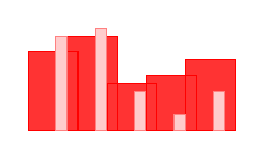
\begin{tikzpicture}[ybar]
		\draw[color=red,fill=red!80,bar width=18pt]
		plot coordinates{(0,1) (.5,1.2) (1,.6) (1.5,.7) (2,.9)};
		\draw[color=red!50,fill=red!20,bar width=4pt,bar shift=3pt]
		plot coordinates{(0,1.2) (.5,1.3) (1,.5) (1.5,.2) (2,.5)};
	\end{tikzpicture}
		
	\section{Conclusion}
	\cite{kamilaris2018deep} WGM evanescent field penetration depth into the cuprous oxide adjacent crystal is much larger than the QE
	radius \citep{mackenzie1992risk,deng2014deep,kamilaris2018deep}:Below we compare the evanescent quadrupole polariton and conventional bulk quadrupole polariton in cuprous
	oxide. \citep{goodfellow2016deep} and \cite{kamilaris2018deep} simplicity let us consider the incident polariton wave vector running along the interface (z direction). The
	polarization of the polariton is taken along the x direction.In this section let us utilize the above calculated WGM-QE interaction to obtain the evanescent polariton (EP)
	
	\bibliography{myRef}
\end{document}